\documentclass[12pt, titlepage]{article}

\usepackage{booktabs}
\usepackage{tabularx}
\usepackage{hyperref}
\hypersetup{
    colorlinks,
    citecolor=black,
    filecolor=black,
    linkcolor=red,
    urlcolor=blue
}
\usepackage[round]{natbib}
\usepackage{graphicx}
\usepackage{float}

\input{../Comments.text}
\input{../Common.text}

\begin{document}

\title{Verification and Validation Report: \progname} 
\author{\authname}
\date{\today}
	
\maketitle

\pagenumbering{roman}

\section{Revision History}

\begin{tabularx}{\textwidth}{p{3cm}p{2cm}X}
\toprule {\bf Date} & {\bf Version} & {\bf Notes}\\
\midrule
2026/04/17 & 1.0 & Initial VnV Report\\
\bottomrule
\end{tabularx}

~\newpage

\section{Symbols, Abbreviations and Acronyms}

See SRS Documentation at \href{https://mei0725.github.io/FlockingSimulator/SRS/SRS.pdf}{SRS}.

\newpage

\tableofcontents

\listoftables %if appropriate

\listoffigures %if appropriate

\newpage

\pagenumbering{arabic}

This document summarized the result of the 
\href{https://mei0725.github.io/FlockingSimulator/VnVPlan/VnVPlan.pdf}{VnV Plan}. 
The requirements that were being tested are detailed in the 
\href{https://mei0725.github.io/FlockingSimulator/SRS/SRS.pdf}{SRS}.

\section{Functional Requirements Evaluation} \label{sec_funcEval}

\subsection{Input Test} \label{inputTest}

These test cases are designed to test the input validation and error handling, 
and they are included in the Unit Test of input UI. Since UI limitations 
prevent invalid method inputs, the test of Integration Methods 
(test-input-method) is not included in it. 

All test cases are passed. 

Test file: \href{https://github.com/Mei0725/FlockingSimulator/blob/main/src/Assets/Tests/IO/InputReaderTests.cs}{InputReaderTests.cs} [VnV Plan 4.1.1]

\subsection{Test of Motion Logic} \label{motionTest}

These test cases are designed to test the correctness of agents' movement logic. 

All test cases are passed. 

Test file: \href{https://github.com/Mei0725/FlockingSimulator/blob/main/src/Assets/Tests/FunctionalTest/FunctionalTest.cs}{FunctionalTest.cs} [VnV Plan 4.1.2]

\subsection{Boundary Testing of Variables} \label{boundaryTest}

These test cases are used to test whether the maximum speed of agents during 
the running of flocking exceeds the limit. 

In this test, only the average speed at each moment was checked. It's because 
checking the velocity of all agents at each time needs to modify the code 
and adds a large number of parameters that are essentially useless for the 
overall running of the program - the speed of each agent at each moment. And 
when the speed explodes, it becomes large enough to affect the average speed 
of the entire flocking.

All test cases are passed. 

Test file: \href{https://github.com/Mei0725/FlockingSimulator/blob/main/src/Assets/Tests/FunctionalTest/FunctionalTest.cs}{FunctionalTest.cs} [VnV Plan 4.1.3]

\subsection{Testing of Integration Methods} \label{methodTest}

These test cases are designed to test if the results of different integration 
method at different timesteps meet expectations. 

In addition to the comparison between timesteps of 0.1s and 0.01s described 
in VnV Plan, an additional comparison was conducted between timesteps of 1s 
and 0.01s. In the former case, a few results did not match expectations. 
For example, the cohesion values produced by RK4 and Implicit Euler showed a 
smaller difference at a timestep of 0.1s. 

There are two possible reasons were identified. First, based on multiple 
previous runs, the RK4 and Implicit Euler methods already tend to produce 
relatively similar results in the flocking simulation. Second, differences 
in timestep size mean that the flocking states cannot be perfectly aligned 
in time. At certain moments, the larger-step simulation may have already 
avoided an obstacle and begun regrouping, while the smaller-step simulation 
may still be in the obstacle-avoidance phase, causing temporary 
inconsistencies to be captured when the timestep difference is not large 
enough. 

But after increasing the timestep to 1s and reducing the testing 
frequency, all checks were successfully passed, which mean at every tested 
moment, the differences between integration methods at a 1s timestep were 
greater than those at a 0.01s timestep.

Test file: \href{https://github.com/Mei0725/FlockingSimulator/blob/main/src/Assets/Tests/FunctionalTest/FunctionalTest.cs}{FunctionalTest.cs} [VnV Plan 4.1.4]

\section{Nonfunctional Requirements Evaluation}

\subsection{Correctness}

The correctness of code is tested through section \ref{sec_funcEval}.
		
\subsection{Verifiability}

The verifiability of this project is guaranteed by 
\href{https://mei0725.github.io/FlockingSimulator/VnVPlan/VnVPlan.pdf}{VnV Plan}
and this document.

\subsection{Usability}

The developer showed a demo during the final presentation and collected the 
usability survey results shown in Figure \ref{FigUsability} based on audience 
feedback.

As shown, the software received relatively high scores for execution speed 
and line chart visualization. However, the overall evaluation and the variable 
input UI received comparatively lower scores. The following additional feedback 
was also provided regarding overall functionality:

\begin{itemize}
\item The uniform red return messages may be associated with errors or warnings.
\item Repeatedly copying file paths reduces usability and efficiency.
\item A zoom function should be desired in the animation display.
\item The line chart should display a y-axis and labels for different lines.
\end{itemize}

The first issue was already solved after the presentation. The third and fourth 
points are existing features: for the third point, the software already 
supports automatic scaling based on agent distribution, but this was not 
demonstrated during the demo. For the fourth point, labels can be displayed 
by hovering the mouse over the corresponding position; they are not shown 
permanently to avoid cluttering the interface. The second point is related to 
the intended design purpose of the software, so no changes are planned at 
this time.

\begin{figure}[H]
\centering
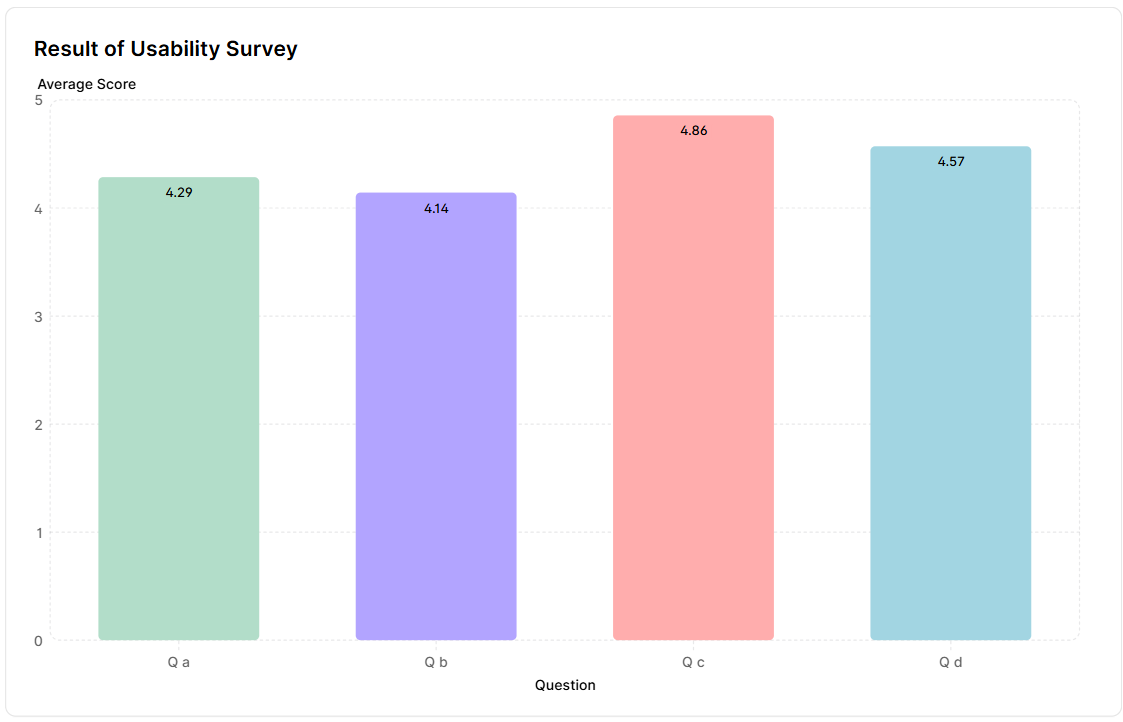
\includegraphics[width=0.9\textwidth]{UsabilityRes.png}
\caption{Result of Usability Survey}
\label{FigUsability}
\end{figure}
		
\subsection{Realism}

The developer showed a demo during the final presentation and collected 
the realism survey results shown in Figure \ref{FigRealism} based on audience 
feedback.

Overall, the software received positive results regarding the realism of the 
simulation. However, due to limitations in both the software itself and the 
survey design, the expected feedback on the realism comparison between 
different integration methods was not obtained. The animation did not include 
labels identifying the different numerical integration methods, making 
comparison difficult for the audience. In addition, because the runtime was 
too short, the effects of different integration methods on the realism and 
stability of the flocking simulation were not clearly demonstrated.


\begin{figure}[H]
\centering
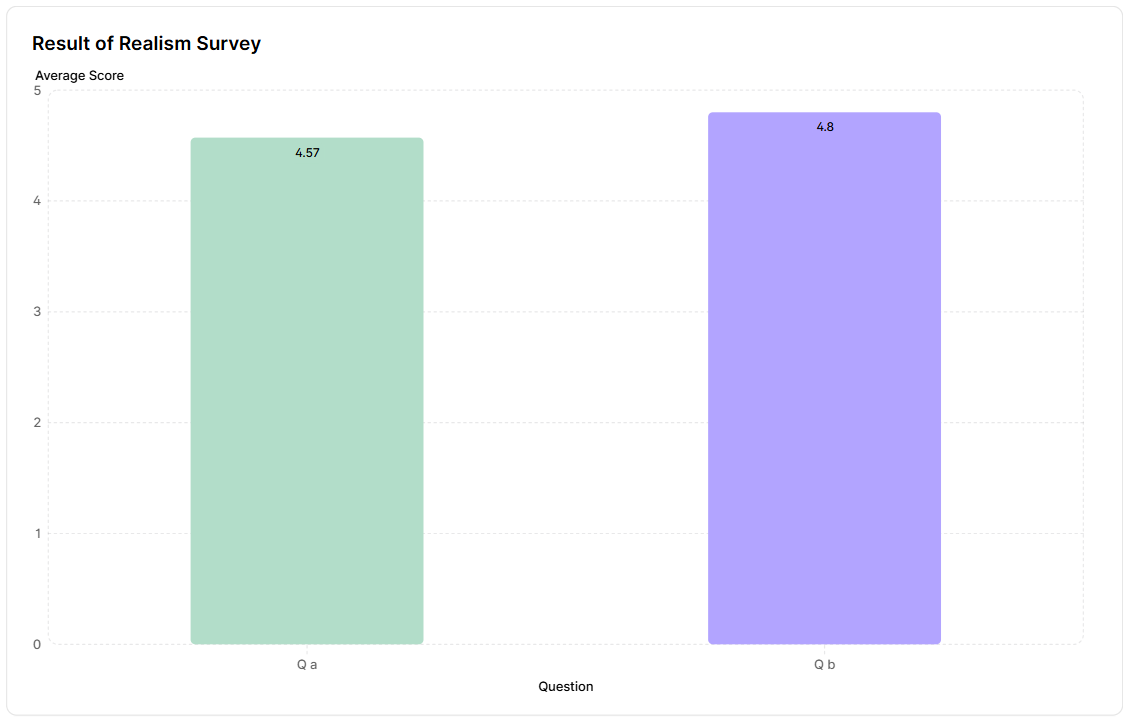
\includegraphics[width=0.9\textwidth]{RealismRes.png}
\caption{Result of Realism Survey}
\label{FigRealism}
\end{figure}

\subsection{Maintainability}

Due to time constraints, the test for developer to add a ODE method is not yet 
performed, but assuming it is, the result shall be presented as:

\begin{itemize}
\item average development time token: x
\item percentage that still passed all tests: x%
\end{itemize}

\section{Unit Testing}

All unit tests for this project have been passed. Through the configured CI 
pipeline, unit tests for the current version of the code can be run from the 
interface at \href{https://github.com/Mei0725/FlockingSimulator/actions/workflows/unity-tests.yml}{GitHub Actions}, 
and the execution summary can be viewed in the `test summary` section of the 
corresponding workflow, and the detailed results can be downloaded from its 
Artifacts.

\section{Changes Due to Testing}

In addition to the bugs identified during testing, two main changes were made 
after the final presentation:

\begin{itemize}
\item The display color for successful results in the graphical interface was 
changed to green, to avoid associations with errors.
\item To make comparisons between different numerical integration methods more 
convenient, the allowed timestep range was expanded from [0.005, 0.1] 
to [0.005, 1].
\end{itemize}

\section{Automated Testing}

The CI pipeline for this project has been configured at 
\href{https://github.com/Mei0725/FlockingSimulator/actions/workflows/unity-tests.yml}{GitHub Actions}, 
to ensure that unit tests and system tests continue to pass after each code 
change. It is automatically triggered whenever files in the /src folder are 
modified, and it can also be triggered manually from the corresponding webpage.

\newpage

\section{Trace to Requirements}

\begin{table}[h!]
\caption{Traceability Between Test Cases and Requirements} \label{tblTraceToRequire} 
\centering
\begin{tabular}{|c|c|c|c|c|c|c|c|c|c|c|c|c|}
\hline
	& R1 & R2 & R3 & R4 & R5 & R6 & R7 & NFR1 & NFR2 & NFR3 & NFR4 & NFR5 \\
\hline
\href{https://github.com/Mei0725/FlockingSimulator/blob/main/src/Assets/Tests/FlockingCalculator/DynamicsTests.cs}{DynamicsTests}
& & & &X& & & & & & & & \\ \hline
\href{https://github.com/Mei0725/FlockingSimulator/blob/main/src/Assets/Tests/FunctionalTest/FlockingMetricsTests.cs}{FlockingMetricsTests}
& & & & &X& & & & & & & \\ \hline
\href{https://github.com/Mei0725/FlockingSimulator/blob/main/src/Assets/Tests/FunctionalTest/ForceTests.cs}{ForceTests}
& & & &X& & & & & & & & \\ \hline
\href{https://github.com/Mei0725/FlockingSimulator/blob/main/src/Assets/Tests/FunctionalTest/ODESolverTests.cs}{ODESolverTests}
& & &X& & & & & & & & & \\ \hline
\href{https://github.com/Mei0725/FlockingSimulator/blob/main/src/Assets/Tests/FunctionalTest/FunctionalTest.cs}{FunctionalTest}
& & &X&X& & & & & & & & \\ \hline
\href{https://github.com/Mei0725/FlockingSimulator/blob/main/src/Assets/Tests/IO/FilesIOTests.cs}{FilesIOTests}
&X& & & & & & & & & & & \\ \hline
\href{https://github.com/Mei0725/FlockingSimulator/blob/main/src/Assets/Tests/IO/InputReaderTests.cs}{InputReaderTests}
&X& & & & & & & & & & & \\ \hline
\href{https://github.com/Mei0725/FlockingSimulator/blob/main/src/Assets/Tests/IO/InputValidationTests.cs}{InputValidationTests}
& &X& & & & & & & & & & \\ \hline
\href{https://github.com/Mei0725/FlockingSimulator/blob/main/src/Assets/Tests/Visualization/AnimationSimulatorTests.cs}{AnimationSimulatorTests}
& & & & & &X& & & & & & \\ \hline
\href{https://github.com/Mei0725/FlockingSimulator/blob/main/src/Assets/Tests/Visualization/ChartDrawerTests.cs}{ChartDrawerTests}
& & & & & & &X& & & & & \\ \hline
Test Correctness        & & & & & & & &X& & & & \\ \hline
Test Verifiability      & & & & & & & & &X& & & \\ \hline
Test Usability          & & & & & & & & & &X& & \\ \hline
Test Realism            & & & & & & & & & & &X& \\ \hline
Test Maintainability    & & & & & & & & & & & &X\\ \hline
\end{tabular}
\end{table}
		
% \newpage

\section{Trace to Modules}		

\begin{table}[h!]
\caption{Traceability Between Test Cases and Modules} \label{tblTraceToModule} 
\centering
\begin{tabular}{|c|c|c|c|c|c|c|c|c|c|c|c|}
\hline
	& M1 & M2 & M3 & M4 & M5 & M6 & M7 & M11 & M12 & M13 & M14 \\
\hline
\href{https://github.com/Mei0725/FlockingSimulator/blob/main/src/Assets/Tests/MainControllerTests.cs}{MainControllerTests}
& &X& & & & & & & & &\\ \hline
\href{https://github.com/Mei0725/FlockingSimulator/blob/main/src/Assets/Tests/FlockingCalculator/DynamicsTests.cs}{DynamicsTests}
& & & & & & &X& & & &\\ \hline
\href{https://github.com/Mei0725/FlockingSimulator/blob/main/src/Assets/Tests/FlockingCalculator/FlockingMetricsTests.cs}{FlockingMetricsTests}
& & & & & &X& & & & &\\ \hline
\href{https://github.com/Mei0725/FlockingSimulator/blob/main/src/Assets/Tests/FlockingCalculator/ForceTests.cs}{ForceTests}
& & & &X& & & & & & &\\ \hline
\href{https://github.com/Mei0725/FlockingSimulator/blob/main/src/Assets/Tests/FlockingCalculator/ODESolverTests.cs}{ODESolverTests}
& & & & &X& & & & & &\\ \hline
\href{https://github.com/Mei0725/FlockingSimulator/blob/main/src/Assets/Tests/FunctionalTest/FunctionalTest.cs}{FunctionalTest}
& & & &X&X&X&X& & & &\\ \hline
\href{https://github.com/Mei0725/FlockingSimulator/blob/main/src/Assets/Tests/IO/FilesIOTests.cs}{FilesIOTests}
& & & & & & & & &X& &\\ \hline
\href{https://github.com/Mei0725/FlockingSimulator/blob/main/src/Assets/Tests/IO/InputReaderTests.cs}{InputReaderTests}
& & & & & & & &X& & &\\ \hline
\href{https://github.com/Mei0725/FlockingSimulator/blob/main/src/Assets/Tests/IO/InputValidationTests.cs}{InputValidationTests}
& & &X& & & & & & & &\\ \hline
\href{https://github.com/Mei0725/FlockingSimulator/blob/main/src/Assets/Tests/Visualization/AnimationSimulatorTests.cs}{AnimationSimulatorTests}
& & & & & & & & & &X&\\ \hline
\href{https://github.com/Mei0725/FlockingSimulator/blob/main/src/Assets/Tests/Visualization/ChartDrawerTests.cs}{ChartDrawerTests}
& & & & & & & & & & &X\\ \hline
\end{tabular}
\end{table}

\newpage

\section{Code Coverage Metrics}

The results of the Code Coverage Metrics are shown in Figure \ref{FigCoverage}, 
and the execution details can also be downloaded from Artifacts at 
\href{https://github.com/Mei0725/FlockingSimulator/actions/workflows/unity-tests.yml}{GitHub Actions}.

The small amount of uncovered code is mainly concentrated in the UI and in 
some error-handling logic that is difficult to trigger.

\begin{figure}[H]
\centering
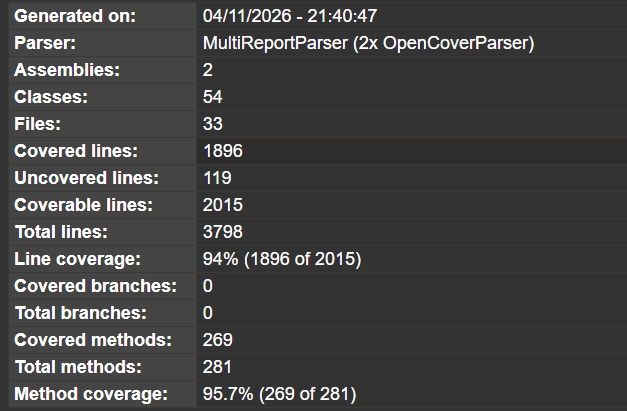
\includegraphics[width=0.9\textwidth]{CodeCoverage.png}
\caption{Code Coverage}
\label{FigCoverage}
\end{figure}

% \section{Extras}

% \wss{Summary of the status of your extras.  If feasible, the extras should be
% complete by the time of writing the VnV report.  If the extras are not complete,
% you should summarize the plans for completing them.}

\bibliographystyle{plainnat}
% \bibliography{../../refs/References}

\newpage{}
\section*{Appendix --- Reflection}

% The information in this section will be used to evaluate the team members on the
% graduate attribute of Reflection.

\input{../Reflection.text}

\begin{enumerate}
  \item What went well while writing this deliverable? 
  
  Thanks to the previously well-prepared VnV Plan and design documents, the 
  overall implementation and testing process went smoothly without major 
  difficulties. This software was developed step by step according to the 
  designed modules, and test cases were implemented based on the original 
  VnV Plan. During this process, several issues were identified through 
  testing and then resolved.
  \item What pain points did you experience during this deliverable, and how
    did you resolve them?

  One of the main challenges during this deliverable was module design. 
  This project contains many features, each relatively small, with some parts 
  that could reasonably be combined or separated. For example, the internal 
  flocking force calculations and the calculations used for displaying flocking 
  metrics are related, but serve different purposes. I considered merging them, 
  but finally kept them separate to preserve modular independence and 
  maintainability.

  Another challenge was designing clear input and output visualization. Since 
  the project produces many outputs and visual comparison is important, it was 
  difficult to present multiple simulation results clearly. To solve this, I 
  collected feedback during both the proof of concept demonstrations and final 
  presentation. Based on that feedback, I added nets and automatic scaling to 
  the animation view, and included additional line charts showing squared 
  differences to make comparisons between simulations more visible.
  \item Which parts of this document stemmed from speaking to your client(s) or
  a proxy (e.g. your peers)? Which ones were not, and why?

  In this document, the following sections were influenced by feedback from 
  the reviewer, professor, and classmates in CAS 741:
  \begin{enumerate}
  \item Based on the professor's suggestion, a single-agent test case was 
  added to the Tests for Functional Requirements section to verify agent 
  behavior in the simplest case.
  \item Based on the professor's suggestion, additional larger-timestep test 
  cases were added to the Testing of Integration Methods section to make 
  differences between methods more visible.
  \item Based on feedback from classmates in CAS 741, usability and realism 
  analyses were conducted, and parts of the visualization were improved 
  accordingly.
  \end{enumerate}
  \item In what ways was the Verification and Validation (VnV) Plan different
  from the activities that were actually conducted for VnV?  

  This VnV Report is generally consistent with the original VnV Plan, with 
  only a few minor differences:
  \begin{enumerate}
  \item Since the UI already restricts the available ODE method selections, 
  invalid method inputs cannot occur, so no additional validation test for the 
  method parameter was performed.
  \item For testing the maximum agent speed limit, the metric was changed from 
  checking each agent's speed at every timestep to comparing the average speed 
  of each flocking simulation at each timestep, avoiding the need for extra 
  parameters with no other use.
  \item To make differences between integration methods more visible, the upper 
  bound of the acceptable timestep range was increased, and test cases with a 
  timestep of 1s were added.
  \end{enumerate}
\end{enumerate}

\end{document}